\documentclass{beamer}

\usepackage[utf8]{inputenc}
\usepackage{default}

\usetheme{CambridgeUS}
%\usecolortheme{seagull}
%\useoutertheme{tree}
\beamertemplatenavigationsymbolsempty
\hypersetup{pdfstartview={Fit}}
\title[Behavior Based Architectures]{Behavior Based Systems}
\author{Luke Fraser}
\date{\today}
\begin{document}

\begin{frame}
 \titlepage
\end{frame}

\begin{frame}{Overview}
 \begin{itemize}
  \item Robot Control Architectures
  \item Behavior Based Systems
  \item Representation
  \item Learning
 \end{itemize}
\end{frame}
\section{Robot Control Architectures}
\begin{frame}{Robot Control Architectures}
 \begin{itemize}
  \item Deliberative - Think, Then Act
  \item Reactive - Don't Think, Act
  \item Hybrid - Think and Act Concurrently
  \item Behavior Based - Think the Way You Act
 \end{itemize}
\end{frame}

\begin{frame}{Deliberative - Think, Then Act}
 \begin{itemize}
  \item Planning
  \item SPA - Sense Plan Act
  \item Pros
  \begin{itemize}
   \item Optimal Solution - \emph{If computationally feasible.}
   \item A good solution in a world that does not change.
  \end{itemize}
  \item Cons
  \begin{itemize}
   \item Slow
   \item Dynamic environments
   \begin{itemize}
    \item Environment will change during deliberation stage.
    \item Solution only correct for previous time-slice.
   \end{itemize}
  \end{itemize}
 \end{itemize}
\end{frame}

\begin{frame}{Reactive - Don't Think, Act}
 \begin{columns}[T]
  \begin{column}[T]{6cm}
  \begin{itemize}
    \item No Planning
    \item No world model
    \item Pros
    \begin{itemize}
    \item Fast
    \item Perform simple tasks well
    \item Emergent behavior
    \end{itemize}
    \item Cons
    \begin{itemize}
    \item No Planning
    \item Limited functionality
    \item Emergent behavior
    \end{itemize}
  \end{itemize}
  \end{column}
  \begin{column}[T]{4cm}
  \centering
   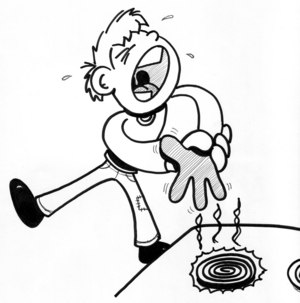
\includegraphics[width=4cm]{stove.jpg}
  \end{column}
 \end{columns}
\end{frame}

\begin{frame}{Hybrid - Think and Act Concurrently}
 \begin{itemize}
  \item Deliberative \& Reactive
  \item Pros
  \begin{itemize}
   \item Fast reaction times
   \item Can perform complex actions.
  \end{itemize}
  \item Cons
  \begin{itemize}
   \item Deliberative and reactive layers interfere.
   \item Intermediate layer is difficult to develop. - Which layer is right?
  \end{itemize}
 \end{itemize}
\end{frame}

\begin{frame}{Behavior Based - Think the Way You Act}
 \begin{itemize}
   \item Network of Behaviors
   \item Behavior nodes interact with other behavior nodes to produce output.
   \item Pros
   \begin{itemize}
     \item Reasoning
     \item Planning
     \item Learning
   \end{itemize}
   \item Cons
   \begin{itemize}
     \item Choosing prevailing behavior can be tricky.
     \item Do not perform extensive planning.
     \item Hard to implement.
     \item Emergent behavior
   \end{itemize}
 \end{itemize}
\end{frame}

\section{Behavior Based Systems}
\begin{frame}{Behavior Based Systems}
 \begin{itemize}
  \item Behaviors are implemented as control laws.
  \item Each behavior can take inputs from the robot's sensors or other modules.
  \item Behaviors can independently:
  \begin{itemize}
    \item Receive input from sensors.
    \item Output actions commands to the same actuators.
  \end{itemize}
  \item Behaviors are simple
  \item Concurrently executed
 \end{itemize}
\end{frame}

\begin{frame}{Example: Behavior-based system}
 \begin{center}
  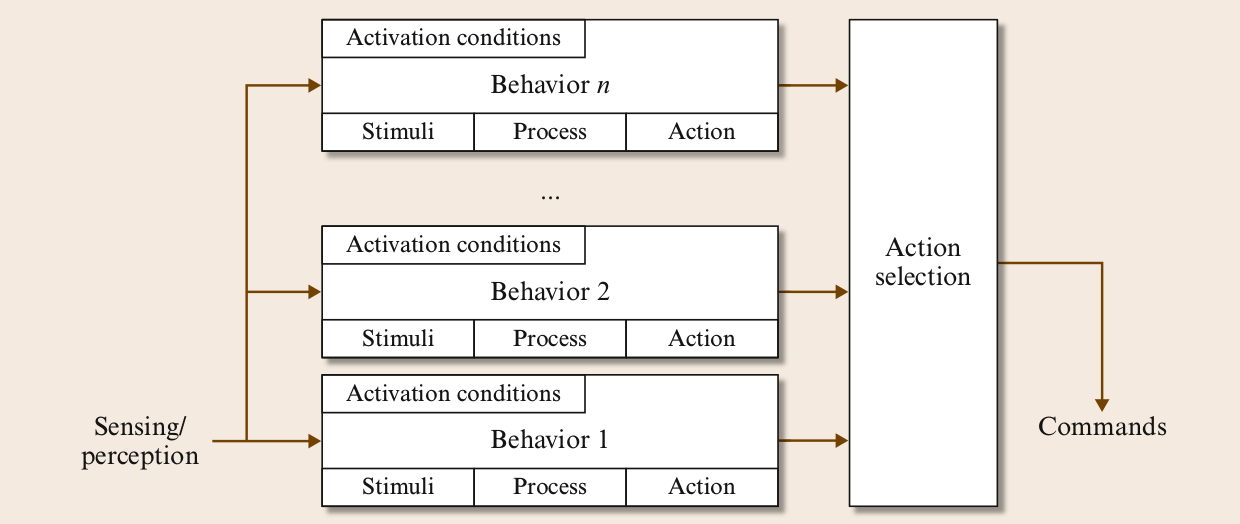
\includegraphics[width=9cm]{behavior_system.png}
 \end{center}
  \end{frame}

\begin{frame}{Example: Behavior-based system}
  Example Behaviors:
  \begin{itemize}
    \item Collision-avoidance
    \item Wall-following
    \item Target-chasing
    \item Find-object
  \end{itemize}
  Example Atomic Actions:
  \begin{itemize}
    \item go-forward-by-a-small-increment
    \item turn-by-a-small-angle
  \end{itemize}
\end{frame}

\begin{frame}{Central Challenge}
 \begin{itemize}
   \item Action Selection/Behavior Coordination
   \begin{itemize}
     \item Behavior hierarchy
     \begin{itemize}
       \item Single parent behavior controls actuator.
     \end{itemize}
     \item Behavior fusion
     \begin{itemize}
       \item Many behaviors together control actuator. \emph{Ex. summing inputs}
     \end{itemize}
     \item Activation spreading
     \begin{itemize}
       \item Behavior with the highest activation energy wins control.
     \end{itemize}
     \item Fuzzy logic/Probability Theory
     \item etc\ldots
   \end{itemize}
  \item Many action selection techniques can be used in the same system.
 \end{itemize}
\end{frame}

\begin{frame}{Misconceptions}
  \begin{itemize}
    \item Easy to implement
    \item Reactive vs. Behavior-based
    \begin{itemize}
      \item Thinking - Achieved through a network of behaviors.
      \item Map storage - distributed over multiple behavior modules.
    \end{itemize}
    \item Hybrid vs.Behavior-based
    \begin{itemize}
      \item Hybrid is more Expressive - They are the same.
      \item Layered systems - Both can be layered.
      \item Hybrid systems - Popular with single robot control.
      \item Behavior systems - Popular with multi-robot control.
    \end{itemize}
  \end{itemize}
\end{frame}

\section{Representation}
\begin{frame}{Toto: Behavior-Navigation System}
 \begin{columns}[T]
  \begin{column}[T]{6cm}
     \begin{itemize}
      \item Behaviors:
      \begin{itemize}
	\item Safe navigation
	\item Landmark detection
	\item Map learning
	\item Path planning
      \end{itemize}
      \item Map representation
      \begin{itemize}
        \item Landmarks stored as behaviors
        \item Distributed system of nodes
        \item System can be repositioned and re-plan in real-time.
      \end{itemize}
    \end{itemize}
  \end{column}
  \begin{column}[T]{4cm}
    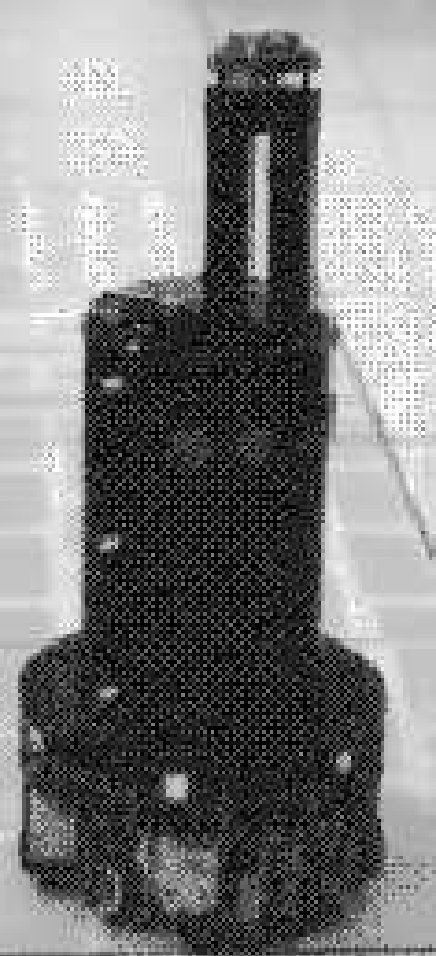
\includegraphics[width=3cm]{toto.png}
  \end{column}
 \end{columns}
\end{frame}

\begin{frame}{Toto: Behavior-Navigation System}
 \begin{itemize}
  \item Landmark goals
  \begin{itemize}
   \item \emph{go to this particular corridor}
   \item \emph{go to the nearest north facing wall}
  \end{itemize}
  \item Message passing - to neighbors
  \begin{itemize}
   \item Activation spreading
   \item Distributed Dijkstra search
  \end{itemize}
 \end{itemize}
\end{frame}

\begin{frame}{Behavior-based Representation: Toto}
 \begin{itemize}
  \item Distributed
  \begin{itemize}
   \item Network of communicating behaviors
   \item Scalable - Adding more nodes to the network doesn't drastically increase computation time
   \item Efficient - Nodes in the graph operate in a distributed manner where there is no centralized controller
  \end{itemize}
 \end{itemize}
\end{frame}

\section{Learning}

\begin{frame}{Learning}
  \begin{itemize}
    \item Goal:
    \begin{itemize}
      \item Reason about a dynamic world quickly
    \end{itemize}
    \item Machine Learning:
    \begin{itemize}
      \item Reinforcement Learning
      \item Evolutionnary computation/Genetic algorithms
      \item Fuzzy Logic
      \item Vision learning
      \item Multi-agent systems
    \end{itemize}
    \item Examples:
    \begin{itemize}
      \item Leanring to walk
      \item Build topo-map
      \item Divide tasks
      \item behave socially
    \end{itemize}
  \end{itemize}
\end{frame}

\begin{frame}{Reinforcement Learning}
  \begin{itemize}  
    \item Goal:
    \begin{itemize}
      \item Improve reinforcement learning through the use of behaviors
      \item Reduce dimensionality of state space through behaviors
    \end{itemize}
    \item Examples:
    \begin{itemize}
      \item Hexapod walking \& Box-pushing
      \begin{itemize}
        \item Decompose into small set of behaviors
        \item Reduced state space
        \item Accelerated and robust learning
      \end{itemize}
      \item Multi-robot systems
      \begin{itemize}
        \item Used Shaping alongside reinforcement learning
      \end{itemize}
    \end{itemize}
    \item Useful for action selection
  \end{itemize}
\end{frame}

\begin{frame}{Learning Behavior Networks}
  \begin{itemize}
    \item Learning at the netowork level
    \begin{itemize}
      \item Abstract behaviors
      \item Primitive behaviors
    \end{itemize}
    \item generalized operator similar to deliberative systems
    \item The robot dynamically learns the task description
    \item Example:
    \begin{itemize}
      \item robot learning a following pattern
    \end{itemize}
  \end{itemize}
\end{frame}

\begin{frame}{Learning from History of Behavior Use}
  \begin{center}
    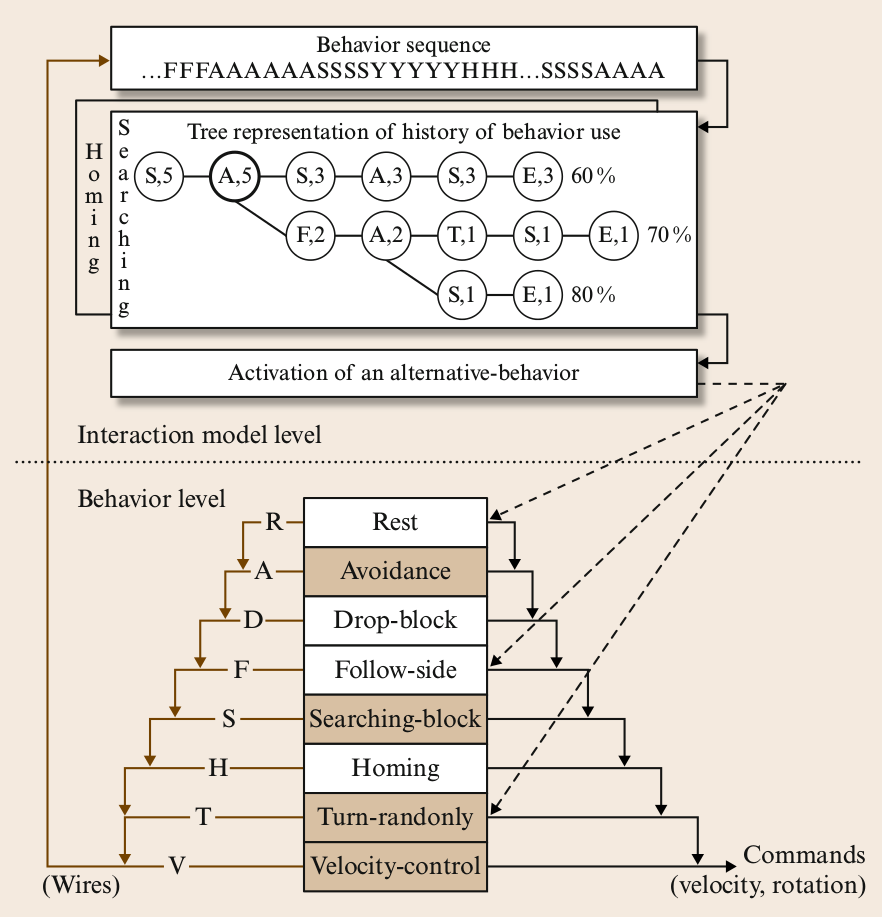
\includegraphics[width=6cm]{history.png}
  \end{center}
\end{frame}

\end{document}
